\section{Modelos Contextuales}

Contexto es tradicionalmente la localizaci\'on, identidad, y estado de las personas, grupos y objetos virtuales y f\'isicos, seg\'un Pereira \cite{pereira2013CSCWD} el contexto puede ser visto como un conjunto de condiciones e influencias en una situaci\'on relevante y que la hacen \'unica y comprensible, esta situaci\'on puede referirse a una persona, grupo de personas, objeto f\'isico, entidad computacional, etc. El concepto de modelos mentales tiene una relaci\'on muy cercana a la consciencia contextual y situacional \cite{aehnelt2012discussion}, al momento de modelar contexto, es necesario distinguir entre los diferentes tipos de informaci\'on contextual\cite{hoyos2013domain}, el contexto de las actividades colaborativas pueden ir desde un editor de documentos distribuido, hasta un videojuego colaborativo; por lo que los elementos particulares de dichas actividades cambia muy radicalmente de uno a otro, y con esto surge la necesidad de usar una taxonom\'ia con un alto nivel de abstracci\'on que soporte la diversidad de contexto con los que se trabaja.

Belkadi et al \cite{Belkadi2013110} proponen un modelo situacional para mejorar la conciencia centrada en los conceptos de situaci\'on, interacci\'on y rol, en el que hacen un recuento de los conceptos clave a tomar en cuenta para un modelo, entre ellos se encuentran: 
\begin{itemize}
\item Elemento contextual
\item Tarea y actividad: describen lo que se espera y lo que se tiene que hacer.
\item Recursos: describe un elemento del contexto, en d\'onde es usado y c\'omo contribuye a la tarea.
\item Interacci\'on: interacciones entre un sujeto y un objeto mediante el uso de herramientas, e interacciones sociales mediante la definici\'on de reglas.
\item Role: definen las responsabilidades de los sujetos.
\end{itemize}

En su modelo para descripci\'on de situaciones definen entidades b\'asicas como recursos humanos y objetos, entidades de interacci\'on que relaciona a las entidades b\'asicas, las cuales se clasifican en cuatro tipos: operacional, que se refiere a las diferentes metas para ser cumplidas(tarea, actividad, proyecto); comunidad, que se refiere a la afiliaci\'on de unas entidades con otras; colaborativa que denota el intercambio de informaci\'on durante una actividad colectiva, y restricciones que indican requerimientos, reglas y l\'imites para la realizaci\'on de una tarea. En cuanto a los roles se definen cinco tipos: actor(\textquestiondown Qui\'en hace qu\'e ?), customer(\textquestiondown Para qui\'en ?), manager(\textquestiondown C\'omo ?), support(\textquestiondown Con qu\'e ?), object(\textquestiondown Sobre qu\'e ?).

As\'i mismo Pereira et. al. \cite{pereira2013CSCWD} maneja un modelo llamado SeCoM(\textit{Semantic Context Model}) dividida en tres capas: ontolog\'ia de alto nivel que representan el contexto o procesos de software, la  ontolog\'ia de integraci\'on es parte de una t\'ecnica para conectar los datos recojidos por los sensores con la arquitectura y la ontolog\'ia de sensores que implementan ontolog\'ias para los datos que son recolectados. El modelo SeCoM consiste de un conjunto modular de ontolog\'ias basadas en dimensiones sem\'anticas de identidad(Actor), ubicaci\'on(Espacio), temporal(tiempo), de actividad(Actividad) y m\'etodos de captura y acceso(Dispositivo).

En otro estudio Alves \cite{alves2013radiator} menciona una definici\'on para los elementos de su modelo definida formalmente como sigue: Un atributo $A_{i}$ es una tupla $( N, V )$, donde \textit{N} es un nombre representando el atributo(por ejemplo, velocidad) y $V$ es el valor del atributo(e.g., 100); $P$ es un conjunto finito de personas ${P_{1},P_{2}...P_{n}}$; $t$ es el rango de tiempo entre dos marcas de tiempo; y $\textit{A}$ un conjunto finito de atributos ${A_{1},A_{2}...A_{n}}$. Con estos elementos representa situaciones definiendo un contexto \textit{C} como una 3-tupla $( P, t, A )$ que representa los atributos que caracteriza la situaci\'on de un grupo de personas $P$ durante un intervalo de tiempo $t$. Por ejemplo suponiendo que Alice est\'a en Nueva York entre Julio 1 y Julio 3. Podemos definir su contexto $C$ como:

$C=( ( Alice ), 01/07..03/07, ( Ubicacion, Nueva York ))$

Este modelo esta orientado a la propagaci\'on despu\'es de que la informaci\'on ha sido agregada tomando en cuenta los atributos en com\'un de las personas que comparten un mismo contexto.

En el trabajo de Ardissono \cite{ardissono2012context} mencionan activity frames para simplificar el contexto de actividades cooperativas, un frame era definido por una 5-tupla $( fn, U, O, Oi, T )$, donde $fn$ era el nombre del frame, $U$ el conjunto de usuarios involucrados en la actividad, $O$ los objetos asociados al frame, $Oi$ es el conjunto de objetos del frame por medio de inferencias, y $T$ las tareas asociadas a la actividad. Y a su vez las tareas est\'an formadas por $( tn, U, O, Oi, g, P, T, s, d )$, donde $tn$ es el nombre de la tarea, $U$, $O$ y $Oi$ como dicho antes son los Usuarios, Objetos, y objetos inferidos asociados a la tarea, $g$ es el objetivo, $P$ es el grupo de tareas que deben de estar cerradas antes de iniciar $tn$, $T$ es el conjunto de tareas hijas, $s$ es el estado(habilitada, deshabilitada, cerrada) y $d$ es la fecha l\'imite para terminar la tarea, nula por defecto.

Anallely Olivares \cite{olivares2011} menciona que es importante tomar en cuenta el contexto de una actvidad colaborativa en lugar de hacerlo para cada uno de los usuarios, es por eso que en su modelo enfatiza el uso de variables t\'ipicas de un grupo de trabajo, por ejemplo estado de los proyectos, pol\'iticas de la organizaci\'on, ubicaci\'on f\'isica de los colaboradores, recursos disponibles, etc.

Bo Hu \cite{bohu2013} divide su modelo en dos partes una meta ontolog\'ia y una ontolog\'ia de dominio,  los elementos del meta modelo se encuentran organizados en cinco categor\'ias: c\'omputo, que define elementos como dispositivos, servicios, redes, y sistemas; persona, con elementos como usuarios, dise\~nadores y desarrolladores; ubicaci\'on, que se divide en la ubicaci\'on f\'isica y distancia; actividad, con dos tipos de actividades, planeadas y no planeadas; y misi\'on, donde se identifican misiones, metas y requerimientos. La ontolog\'ia espec\'ifica de dominio define los conceptos y relaciones dentro del dominio dado, y es restringido por el meta modelo.

En el a\~no 2013 se propone MARS que es un modelo contextual de regulaci\'on que ayuda a modelar la actividad soportada por herramientas groupware. En este modelo las interacciones toman lugar en un espacio llamado arena, cada interacci\'on es representada por un escenario que describe la forma en que se lleva a cabo dicha interacci\'on, qui\'enes participan y los objetos involucrados, adem\'as se definen condiciones y precondiciones para que este escenario se lleve a cabo; en esta arena est\'an presentes actores que realizan acciones, durante esta actividad se manejan o producen objetos; actores y objetos pertenecen a diferentes familias y desempe\'nan diferentes papeles o roles. Dado que los miembros de un grupo colaborativo pueden serlo a su vez de otro, se definen vistas que determinan los actores, objetos e interacciones que una arena puede compartir con otra.

En otro caso Montan\'e et. al. proponen un modelo de contexto social\cite{montane2013context}, donde hay categor\'ias similares, tomando en cuenta las relaciones entre los sujetos adem\'as de las actividades y estado actual de cada uno de ellos; los elementos que lista en su trabajo est\'an divididos en tres categor\'ias. La interactiva describe a los usuarios de forma individual y sus interacciones con las cosas que los rodean como objetos, tareas, eventos, usuarios o ubicaciones; la cohesiva integra elementos que tienen que ver con la actividad grupal y se pueden encontrar los grupos, roles, metas, alianzas, actividades y reglas. Y las afectivas que describen c\'omo se sienten los miembros del grupo al realizar las actividades entre ellas est\'an los sentimientos y los gestos.	

Skillen \cite{Skillen201497} habla de un mecanismo de personalizaci\'on basado en reglas donde identifica conceptos clave para modelar a los usuarios en un ambiente pervasivo de los que lista los siguientes: Usuario, Perfil de usuario, ubicaci\'on, preferencias del usuario, Objeto de asistencia en una interacci\'on, actividad que realiza el usuario, contenido multimedia que ser\'a enviado al usuario(audio, video, imagen o texto), Condici\'on de salud que pueden afectar el tipo de medio que se le env\'ia al usuario, escala de calidad de la informaci\'on entregada, y formato de interfaz de usuario donde se desplegar\'a la informaci\'on enviada.

En una revisi\'on de la literatura sobre modelos contextuales se revisaron ontolog\'ias contextuales, entre las que se pod\'ian encontrar los siguientes elementos:

\begin{center}
\begin{longtable}{|p{3cm}|p{10cm}|}
\caption{Unidades contextuales encontradas en los frameworks revisados.}\\
\hline
\textbf{Elementos} & \textbf{Descripci\'on}\\
\hline
\endfirsthead
\multicolumn{2}{c}%
{\tablename\ \thetable\ -- \textit{Contin\'ua de p\'agina anterior}} \\
\hline
\textbf{Elementos} & \textbf{Descripci\'on} \\
\hline
\endhead
\hline \multicolumn{2}{r}{\textit{Contin\'ua en siguiente p\'agina}} \\
\endfoot
\hline
\endlastfoot

	Objetos o artefactos & Entidades sobre las que los usuarios pueden realizar alguna acci\'on. \\
	\hline
	Tareas & Acciones asociadas con usuarios, objetos, objetivos y subtareas que se deben de llevar a cabo para alcanzar un objetivo. \\
	\hline
	Eventos & Eventos ocurridos en interacciones\cite{montane2013context}\\
	\hline
	Usuarios & Entidades que pertenecen a una comunidad y que realizan tareas\cite{montane2013context}. \\
	\hline
	Ubicaciones & Posici\'on virtual o f\'isica en un grupo \cite{montane2013context}. \\
	\hline
	Grupos & Colecci\'on de usuarios que realizan una actividad\cite{montane2013context}. \\
	\hline
	Objetivos & Los objetivos de la comunidad\cite{montane2013context}. \\
	\hline
	Alianzas & Subconjunto de usuarios en un grupo \cite{montane2013context}. \\
	\hline
	Actividades & Actividades realizadas por un grupo\cite{montane2013context}. \\
	\hline
	Reglas & Comportamientos definidos por el grupo \cite{montane2013context}. \\
	\hline
	Foco de visi\'on & D\'onde est\'an mirando los usuarios\cite{gallardo2012framework}. \\
	\hline
	Vistas de sistema, espacios de trabajo & Qu\'e pueden ver los usuarios \cite{gallardo2012framework}. \\
	\hline
	Alcance & Alcance de los usuarios\cite{gallardo2012framework}. \\
	\hline
	Presencia & Presencia de usuarios en el espacio de trabajo\cite{gallardo2012framework}. \\
	\hline
	Intenci\'on & De qu\'e objetivo es parte una tarea\cite{gallardo2012framework}. \\
	\hline
	Habilidades & Capacidad para llevar a cabo un conjunto de actividades con cierto nivel de destreza \cite{decouchant2013adapting}. \\
	\hline
	Contexto f\'isico & Incluye todas las magnitudes f\'isicas (e.g. tiempo, espacio, temperatura, nivel de luz, nivel de ruido)\cite{hoyos2013domain}. \\
	\hline
	Contexto computacional & Informaci\'on relacionada con el software y hardware de sistemas, e.g. trafico de red, condiciones, estatus de hardware, informaci\'on pedida por el usuario, requerimientos de memoria\cite{hoyos2013domain}. \\
	\hline
	Ambiente & Descripci\'on de la distribuci\'on f\'isica de los objetos y usuarios en un espacio de trabajo\cite{hoyos2013domain}. \\
	\hline
\end{longtable}
\end{center}

Todos estos elementos se extrajeron de diferentes modelos entre los que se hizo la siguiente tabla comparativa:

\begin{figure}[h!]
  \centering
    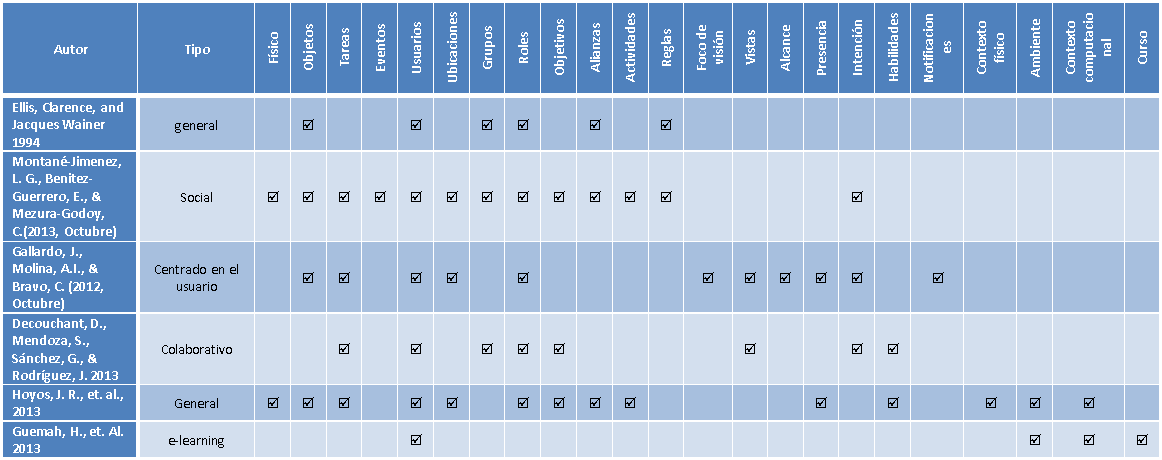
\includegraphics[scale=0.5]{cmpcntx}
  \caption{Comparaci\'on de modelos de contexto\cite{ellis1994conceptual}\cite{montane2013context}\cite{gallardo2012framework}}
\end{figure}

% % % % % % % % % % % % % % % % % % % % % % % % % % % % % % % % % % % % % % % % % % % % % % % % % % % % % % % % % % % % %

\section{Arquitecturas y Marcos de Trabajo Conscientes del Contexto}

Gutheim \cite{gutheim2011} menciona que hay dos tipos de arquitecturas, las que siguen un modelo distribuido haciendo uso de servicios(\textit{broker}) usado tradicionalmente para decoplar proveedores y consumidores de datos contextuales, este modelo es usualmente utilizado para  modelar contexto y para mecanismos de inferencia; el otro tipo de arquitecturas son aquellas que siguen un modelo punto a punto en el que generalmente los proveedores y consumidores de informaci\'on contextual se conocen mutuamente y se env\'ian informaci\'on directamente \cite{yoosoo2010}.

Para que una arquitectura sea consciente del contexto debe de cumplir con los siguientes requerimientos\cite{dey1999architecture}:

\begin{itemize}
\item Permitir a las aplicaciones acceder a informaci\'on contextual desde m\'aquinas distribuidas en el de la misma forma en que acceden a la entrada del usuario en una m\'aquina local.
\item Soportar la ejecuci\'on de diferentes plataformas y el uso de diferentes lenguajes de programaci\'on.
\item Soportar la interpretaci\'on de informaci\'on contextual.
\item Soportar la agregaci\'on de informaci\'on contextual
\item Soportar independencia y persistencia de widgets contextuales
\item Soportar el almacenamiento del historial de contexto
\end{itemize}

Tambi\'en para el soporte de consciencia contextual, Elg Ghayam \cite{el2011distributed} menciona 2 requerimientos que se deben de cumplir: la formalizaci\'on de contexto, para delimitar los datos contextuales y facilitar la distinci\'on de par\'ametros de contexto, una categorizaci\'on de datos contextuales es requerida, m\'as aun, para reducir la complejidad de su manutenci\'on, una representaci\'on formal tambi\'en es necesaria. El otro punto son reglas de adaptaci\'on: la adaptaci\'on de contexto debe de ser vista como un conjunto de reglas que controlan y anticipan el cambio de contexto que puede ocurrir en el ambiente, por lo tanto, en la construcci\'on de reglas de adaptaci\'on, el n\'umero de par\'ametros contextuales es grande y as\'i, no es evidente que no se pueden enumerar todas las posibles situaciones que van a ocurrir. Por lo anterior, un m\'etodo para construir reglas de adaptaci\'on es requerido, que pueda manejar la diversidad de posibles situaciones que se construyen en base de esos par\'ametros contextuales.

Para poder mejorar la colaboraci\'on de los usuarios, la arquitectura debe de permitir que el groupware pueda adaptarse al contexto, y de acuerdo a Abowd\cite{abowd1999towards} hay 3 tipos de adaptaci\'on:
\begin{itemize}
\item  Presentaci\'on de informaci\'on y servicios al usuario. Se refiere a la t\'ecnica de interacci\'on que muestra una lista de objetos o lugares cuyos elementos m\'as importantes son resaltados de acuerdo al contexto actual del usuario.
\item Ejecuci\'on autom\'atica de un servicio. En este caso un servicio es autom\'aticamente lanzado si la combinaci\'on correcta de condiciones es dada.
\item Aumento de la informaci\'on. Informaci\'on contextual puede servir para entender mejor el ambiente colaborativo.
\end{itemize}

Chihani \cite{Chihani201459} propone un framework que desacopla el manejo de contexto de la l\'ogica de negocio de las aplicaciones siguiendo un modelo \textit{broker}, esta arquitectura consta de 3 capas, los proveedores de informaci\'on contextual, el mecanismo para el manejo de contexto y a los consumidores. En la capa de proveedores se encuentra una funci\'on ``provide" que genera la informaci\'on contextual prima, despu\'es est\'a la capa de manejo de contexto en la que se implementan cuatro funciones para el uso de contexto; la funci\'on de filtrado ``filter" que procesa se\~nales para eliminar el ruido en la informaci\'on contextual, la funci\'on ``abstract" que transforma la informaci\'on contextual prima a un nivel m\'as alto de abstracci\'on en la que se usa un aut\'omata de estado finito compuesto por los estados de los datos contextuales; la funci\'on ``select" que permite la selecci\'on de la ``mejor" informaci\'on contextual basada en criterios programados; y la funci\'on ``aggregate" que realiza una agregaci\'on de informaci\'on contextual basada en un conjunto de reglas que apuntan condiciones que la informaci\'on tiene que cumplir antes de ser consumida. Con respecto de la capa de consumidores, se hace uso de una funci\'on ``consume" la cual accede a la informaci\'on contexual de cualquier nivel(prima, abstracta o compuesta). Una caracter\'istica que diferenc\'ia esta arquitectura de otras es la falta de un modelo contextual con el cual describa la situaci\'on de los usuarios.

Skillen et. al. \cite{Skillen201497} proponen una arquitectura distribuida orientada a servicios para ambientes pervasivos, consta de cuatro componentes que interact\'uan unos con otros para lograr la personalizaci\'on de servicios de asistencia a la orden, el objetivo de esta arquitectura es permitir un flujo de informaci\'on entre una aplicacion y los servicios de ayuda, entre los componentes se encuentran el ambiente pervasivo que es la que genera y consume la informaci\'on  contextual, capa de servicios de perfil de usuarios donde se modela al usuario y sus preferencias, la capa de personalizaci\'on de servicios que consiste de un mecanismo basado en reglas y de inferencia y los servicios de asistencia a la orden que ayudan a los usuarios a manejar sus actividades diarias.

La propuesta de Anallely olivares et. al. \cite{olivares2011} es una arquitectura para soportar el uso de contexto en herramientas groupware basada en escenarios y situaciones que sirven de medios para validar su funcionalidad. Esta arquitectura consiste en cuatro fases: percepci\'on de eventos contextuales divididos en dos tipos: f\'isicos y l\'ogicos, los f\'isicos son recuperados por sensores y los l\'ogicos reflejan cambios en las dimensiones internas del ambiente colaborativo, como el estado de los proyectos; detecci\'on de la situaci\'on donde se le da forma a la informaci\'on recuperada en la fase anterior, para la definici\'on de situaciones se tomaron en cuenta elementos como nombre, entidad afectada por la situaci\'on, oyentes que activan o desactivan situaciones, eventos contextuales que pueden provocar la activaci\'on o desactivaci\'on de situaciones y condiciones que son verificadas antes de activar o desactivar una situaci\'on; la siguiente fase es de comunicaci\'on de la situaci\'on que sigue un modelo suscriptor publicador donde un agente publica la informaci\'on y el suscriptor toma la que es de su inter\'es; la \'ultima fase es adaptaci\'on del sistema en el que usan reglas est\'aticas de la forma \textbf{if} situaci\'on detectada \textbf{then} adaptaci\'on planeada.

Pereira et.al. \cite{pereira2013CSCWD} muestra una arquitectura que sigue un dise\~no multiagentes, dirigida a grupos de trabajo de desarrollo de software, en la que integra herramientas web, una de manejo de proyectos como aplicaci\'on como ambiente de soporte para las actividades de los desarrolladores y otra para control de versiones, ambas herramientas son reguladas por un agente, en esta plataforma se definen dos tipos de agentes: agentes de servicio y asistentes personales; cada usuario cuenta con un asistente que cumple con varias funciones: entender sus necesidades, actuar de manera proactiva para anticiparlas, ejecutar comandos dados por los usuarios, presentar la informaci\'on de forma inteligente, mediar la comunicaci\'on con otros miembros del equipo, y capturar y representar las operaciones de los miembros del equipo ayud\'andolos en el proceso de crear conocimiento. Por otro lado, los agentes de servicio se encargan de encapsular las aplicaciones con las que interactuan los usuarios(la plataforma web de desarrollo y el controlador de versiones) checando las modificaciones en los contenidos de las aplicaciones o actualizando documentos.

El trabajo actual se basa en un trabajo previo de Montan\'e \cite{montane2013context}, en el que, a partir de variables contextuales observadas en experimentos realizados, se propone un modelo conceptual de una arquitectura capaz de trabajar con informaci\'on contextual. La arquitectura se divide en 3 capas: la de adquisici\'on de datos, que es la que recibe los datos por separado dependiendo de la categor\'ia a la que pertenezcan; la de manejo de contexto, que es la capa encargada de administrar el almacenamiento, recuperaci\'on y actualizaci\'on de los datos contextuales que se guardar\'an en una base de datos; y la capa de uso de contexto, que tiene 2 tareas principales: razonar los datos contextuales recuperados, y a partir del resultado obtenido de este procesamiento, entregar informaci\'on relevante a los usuarios de un groupware o enviar instrucciones de ejecuci\'on al sistema para poder adaptarse al contexto de los usuarios.

\begin{figure}[h!]
  \centering
  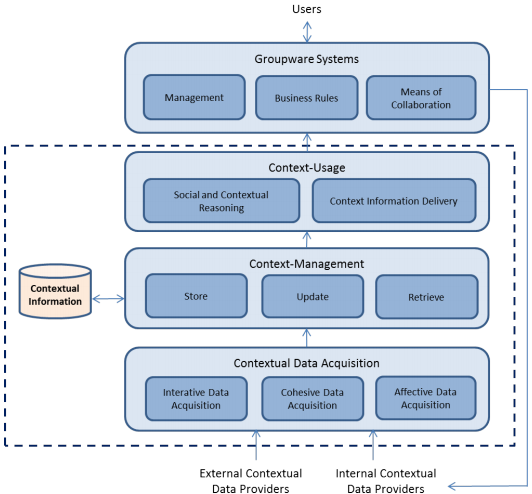
\includegraphics[scale=0.6]{arch}
  \caption{Arquitectura para soportar colaboraci\'on en groupware conscientes del contexto \cite{montane2013context}}
\end{figure}

Muchas arquitecturas se han propuesto para poder soportar sistemas conscientes del contexto, la siguiente tabla hace una comparaci\'on de los elementos y capas de algunas arquitecturas conscientes del contexto, entre las cuales se encuentran la arquitectura base para el presente trabajo que usa un modelo contextual colaborativo clasificado en tres categor\'ias: elementos cohesivos, elementos interactivos y elementos afectivos. La arquitectura de Dey\cite{dey1999architecture}  usa widgets para la captura de datos contextuales y servicios de agregaci\'on de contexto as\'i como servicios de distribuci\'on y razonamiento contextual. En el marco de trabajo de Kamoun \cite{kamoun2012fadyrcos}  se reconfiguran servicios para adaptarlos a situaciones que cambian din\'amicamente. Decouchant \cite{decouchant2013adapting} divide su arquitectura en tres capas: la capa de espacio de trabajo, la de adaptaci\'on y la de detecci\'on de informaci\'on contextual. Guerman  \cite{guermah2013ontology} que propone una arquitectura orientada a sistemas de aprendizaje electr\'onico. En la figura \ref{cmp:fig} se comparan algunos elementos que poseen dichas arquitecturas, entre ellos se encuentran la presencia de capas como adquisici\'on, manejo y distribuci\'on de datos contextuales, persistencia de datos y su reuso, apoyo con v\'ias de comunicaci\'on, el uso de widgets como comunicadores entre el sistema y la arquitectura, manejo de sesiones, esquemas conceptuales de colaboraci\'on, agregaci\'on de datos y la representaci\'on de espacios de trabajo como parte de la arquitectura.

\begin{figure}[h!]
  \centering
    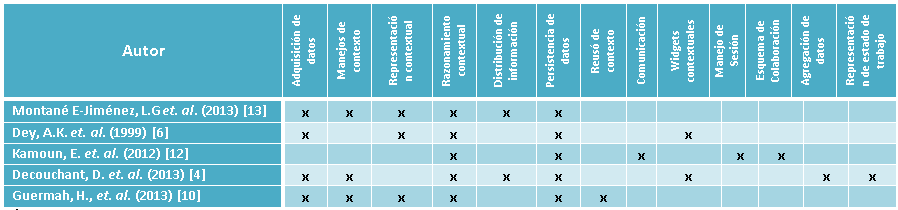
\includegraphics[scale=0.7]{images/comparaciones.png}
  \caption{Comparaci\'on de arquitecturas que soportan consciencia del contexto\cite{montane2013context}\cite{dey1999architecture}\cite{kamoun2012fadyrcos}\cite{decouchant2013adapting}\cite{guermah2013ontology}}
  \label{cmp:fig}
\end{figure}

Dentro las arquitecturas vistas, se identifica un proceso donde la informaci\'on contextual es tratada desde su adquisici\'on hasta la entrega de resultados a las aplicaciones consumidoras.

\subsection{Proceso}

Para obtener resultados de un conjunto de variables contextuales se establecen 3 pasos ya descritos antes \cite{montane2013context}: recuperar las variables contextuales en un formato legible para la computadora, almacenar, recuperar y actualizar los datos contextuales de una base de datos, e inferir resultados de un conjunto particular de variables asociadas unas con otras para despu\'es distribuirlos.

\subsubsection {Adquisici\'on}
El problema de mantener la consciencia del espacio de trabajo en los groupware gira en torno a la obtenci\'on de informaci\'on \'util m\'as que el c\'omo la utilizan los usuarios \cite{ardissono2012context}. Antunes propone un marco de trabajo para evaluar groupwares \cite{antunes2008structuring}, un enfoque entrada-procesamiento-salida para conceptualizar las relaciones entre el soporte tecnol\'ogico y factores relacionados al comportamiento del grupo y contexto de trabajo. Las variables contextuales son factores importantes para describir el comportamiento del grupo, est\'an clasificadas en 5 categor\'ias generales \cite{antunes2008structuring}: personales, situacionales, estructura del grupo, caracter\'isticas de la actividad o tarea y caracter\'isticas tecnol\'ogicas. Los procesos grupales est\'an definidas como las caracter\'isticas de las interacciones del grupo, incluyendo las decisionales, comunicacionales, e interpersonales. Por \'ultimo este framework eval\'ua los resultados de los procesos grupales afectados por el soporte tecnol\'ogico, incluyendo los relacionados con las actividades y con el grupo en s\'i.

\subsubsection {Manejo de contexto}

Alves \cite{alves2013radiator} propone un mecanismo de agregaci\'on de informaci\'on contextual para mejorar la eficiencia de consumo de recursos de red para aplicaciones conscientes del contexto, definiendo agregaci\'on como ${ ( P_{1},t_{1},A_{1} ),..., ( P_{n},t_{n},A_{n} ) }$ es un conjunto de contextos y $Ac$ un atributo en com\'un tal que para todo atributo $A_{i}$ perteneciente a $A_{1} ... A_{n}$, $Ac$ pertenece a $A_{i}$.

$Aggr( A_{c}, {( P_{1},t_{1},A_{1} ),..., ( P_{n},t_{n},A_{n} )}) = ( P, t, A )\Rightarrow \forall P_{i}\in P_{1}...P_{n}:P_{i}\in P \wedge \forall t_{i} \in t_{1}...t_{n}:t_{i}\subseteq t \wedge \forall A_{i}\in A_{1}...A_{n}:A_{i}\in A$

AYPUY es un manejador de recursos creado para ambientes de colaboraci\'on distribuidos.  Almacena diferentes tipos de recursos, como contratos, historias cl\'inicas, objetos de aprendizaje, etc., y garantiza su acceso cumpliendo con los objetos de confidencialidad, seguridad y escalabilidad de los sistemas que lo utilizan. En este framework un recurso est\'a compuesto de un conjunto de atributos $A = { L, D, F }$, donde $L$ describe las caracter\'isticas l\'ogicas generales del recurso (fecha de creaci\'on, autor, tipo de recurso), $D$ establece las caracter\'isticas relacionadas con el dominio (e.g., salud, educaci\'on) al que pertenece el recurso, y $F$ describe las caracter\'isticas f\'isicas de almacenamiento del recurso (e.g., tipo de replicaci\'on, cadena de conexi\'on), as\'i AYPUY establece la estrategia de almacenamiento y acceso, adicionalmente los recursos tienen un conjunto de operadores $O$, que determinan las acciones que se pueden hacer con ellos, y son extensibles para soportar un dominio espec\'ifico.

AYPUY administra los recursos controlando su acceso con espacios de trabajo (ET), crea un ET general al que pertenecen todos los usuarios del sistema siguiendo un rol espec\'ifico, si se requiere la especializaci\'on o modificaci\'on de los roles de acceso a los recursos para todos o un subconjunto de usuarios, se crea otro ET. En un ambiente empresarial, por ejemplo, el ET general representa a la empresa, y un ET1 corresponder\'ia a un departamento y ET1.1 a un proyecto en espec\'ifico.

\subsubsection{Distribuci\'on}
La informaci\'on que se recopila se ocupa de qui\'en est\'a trabajando en un contexto compartido, qu\'e est\'an haciendo, d\'onde est\'an trabajando, cu\'ando ocurren varios eventos, y como suceden esos eventos \cite{ardissono2012context}. La presentaci\'on de informaci\'on consciente es una parte importante de los groupware, Gross\cite{gross2013supporting} menciona los siguientes puntos importantes que se deben de tomar en cuenta al momento de presentar informaci\'on al usuario:
\begin{itemize}
\item La identificaci\'on y el se\'nalamiento de retos sobre la desorganizaci\'on de contenedores de informaci\'on consciente son requerimientos centrales para el apoyar la consciencia.
\item Los sistemas deben de proporcionar sugerencias que los usuarios puedan sobrescribir, ya sea en un momento espec\'ifico o como regla general.
\item La presentaci\'on de informaci\'on de consciencia debe de ser explorada con la participaci\'on del usuario, el tipo de visualizaci\'on de consciencia debe de ajustarse a la necesidad de informaci\'on del usuario y a su contexto.
\item Modelos de consciencia son importantes para estructurar informaci\'on de consciencia
\end{itemize}

Alves \cite{alves2013radiator} propone un modelo gen\'erico para propagaci\'on de contexto (Radiator) y necesidades de privacidad de aplicaciones distribuidas conscientes del contexto, enfocado a mejorar la escalabilidad de las aplicaciones y brindar privacidad de la propagaci\'on de la informaci\'on, adem\'as agrega que la escalabilidad y la privacidad se pueden asegurar retrasando la propagaci\'on de contexto hasta que ciertas condiciones son alcanzadas y entonces agregar los mensajes en niveles sint\'acticos y sem\'anticos, antes de propagar la informaci\'on los datos tienen que tener un nivel de agregabilidad determinado de donde  $CP$ es el contexto actual de una persona $P$ y $C_{x}$ el contexto de alguien m\'as que el sistema quiere propagar a $P$, $G( CP, C_{x} )$ representa que tan agregado debe de estar $C_{x}$ antes de ser transmitido a $P$ , tomando en consideraci\'on el contexto actual de $CP$. Por lo tanto un conjunto de contextos $C_{1}..C_{n}$ es solo propagado a $P$ cuando para todo $i$ perteneciente a $1..n$, $G( CP, C_{i} ) = n$, $n$ siendo un entero. Informalmente la agregabilidad representa el n\'umero de mensajes de contexto que deben de ser retenidos antes de su propagaci\'on, si se define una funci\'on $G$ que siempre regrese 4, el sistema siempre va a agregar cuatro mensajes contextuales antes de propagarlos

En el trabajo de Ardissono \cite{ardissono2012context} se mencionan 2 pol\'iticas dependientes del contexto para el manejo de notificaciones que apoya la selecci\'on de notificaciones para ser entregadas en base a las actividades actuales del usuario en diferentes niveles de granularidad: colaboraci\'on general de la tarea actual del usuario contra tarea llevada a cabo. Estas pol\'iticas son ofrecidas por el framework CONRAD (COntext depeNdent awaReness informAtion Delivery, por sus siglas en ingl\'es). Las 2 pol\'iticas son las siguientes:

\begin{enumerate}
\item el filtro de contexto informa al usuario sobre eventos referentes a los contextos de colaboraci\'on en los que est\'a trabajando e ignora los dem\'as
\item el filtro de tareas es m\'as selectivo y filtra las notificaciones basado en la tarea actual del usuario
\end{enumerate}

Con este framework se reduce el nivel de distracci\'on y la carga de trabajo presentada al usuario al momento de obtener informaci\'on relacionada con su actividad.
El objetivo de su trabajo es proveer a usuarios apoyo automatizado para especificar el tipo de informaci\'on consciente m\'as apropiado basado en la actividad del usuario y ajustar la entrega de las notificaciones y la aplicaci\'on de filtros para preferencias individuales de notificaci\'on.

Para adaptar servicios cooperativos al contexto del usuario, AYLLU \cite{arias2012platform} usa el framework AES que adapta la informaci\'on en diversos contextos. AES funciona de la siguiente manera: una aplicaci\'on env\'ia una consulta inicial a AES para que esta la enriquezca, AES obtiene los perfiles o caracter\'isticas de la aplicaci\'on externa (usuario, contexto, dispositivo, perfiles), e invoca funciones de filtro de acuerdo a los perfiles. El resultado es un conjunto de datos de alta abstracci\'on que es usado para generar una consulta enriquecida que ser\'a devuelta a la aplicaci\'on externa.

El framework AYLLU \cite{arias2012platform} usa un protocolo de comunicaci\'on donde los mensajes son enriquecidos sem\'anticamente, como en un sistema multiagentes. Se basa en la creaci\'on de una serie de agentes, que ayuden al usuario a seguir una serie de protocolos de interacci\'on que determinan un servicio cooperativo, cuando un servicio cooperativo se instancia se crea un Agente Manejador de Comunidad (CMA) por medio de un agente de f\'abrica (FA). Los CMA crean agentes de comunidad (CA) los cuales ejecutan protocolos de interacci\'on comunicacion estructurada entre los CA dentro de un servicio cooperativo. El agente administrador (AA) administra a los usuarios, roles, habilidades, recursos y grupos de trabajo. FA crea los servicios cooperativos en la plataforma, para ejecutar un servicio cooperativo se construye un CMA y un grupo de CA, el CMA controla la creaci\'on, destrucci\'on e interacci\'on  de los CA para informar el estado actual del servicio. Para cada usuario existen dos agentes: el manejador de sesi\'on (SM) y el agente representante (RA), adem\'as cuentan con un agente de interfaz (IA) en cada dispositivo en el que el usuario ejecute un cliente; el SM act\'ua como un puente entre el usuario y los agentes CA asociados con los servicios cooperativos de los que el usuario forma parte, el SM controla los mensajes de cada CA en los servicios cooperativos y los transmite al RA, el cual responde en nombre del usuario a diferentes peticiones, si el RA no puede manejar la informaci\'on, se comunica con el IA para mostrar las peticiones al usuario y le solicitar\'a una respuesta.

\subsubsection{Mecanismos de razonamiento}

Para adaptar los sistemas es necesario reconocer la situaci\'on de los usuarios y saber c\'omo brindarles apoyo, en consecuencia se requiere de una forma de interpretar las interacciones que se est\'an llevando a cabo en la aplicaci\'on con lo que se han propuesto diferentes mecanismos de razonamiento para estos casos.

En el modelo contextual MARS se usa un lenguaje de regulaci\'on para describir escenarios llamado CORAL\footnote{Collaborative Regulation Language} que toma en cuenta tres aspectos de los escenarios definidos en MARS especificados en las pre y pos condiciones de la interacci\'on: qui\'en puede participar en la interacci\'on, qu\'e objetos pueden ser manipulados, qu\'e rol tiene un actor u objeto durante la interacci\'on y en casos similares, referencias a otros escenarios. Con esto se define el lenguaje CoRaL con la siguiente sintaxis descrita en noteaci\'on BNF. Siendo E el conjunto de elementos de cadenas de nombres de arenas, actores, familias de actores, familias de objetos, objetos y roles:
	
\begin{gather*}
 \langle sentencia \rangle ::= \langle expresi\acute{o}n \rangle \langle operador \rangle \langle expresi\acute{o}n \rangle";"\\
 \langle expresi\acute{o}n \rangle  ::= \langle palabraReservada \rangle :\{\langle elementos \rangle \}\\
 \langle expresi\acute{o}n \rangle  ::=! \langle palabraReservada \rangle :\{\langle elementos \rangle \}\\
 \langle operador \rangle  ::=  :: | \rightarrow  \\
 \langle palabraReservada \rangle  ::= "Arena" |\\* "Interacci\acute{o}n" | "Actor" | "Familia de actor" \\*| "Familia de Objeto" | "Objeto" | "Rol"\\
 \langle elemento \rangle  ::= cualquier cadena en E
\end{gather*}

Skillen \cite{Skillen201497} en su capa de uso de contexto define cuatro funciones para el procesamiento de contexto, estas funciones se definen con el lenguaje de reglas de web semantico SWRL con el que describe condiciones que la informaci\'on contextual debe de cumplir para personalizar un conjunto de servicios. Haciendo uso de la sintaxis de este lenguaje definen reglas como la siguiente. $UserProfile(?up), hasHealthCondition(?up, Blind) \rightarrow HelpDelivery(PlayAudio), hasMediaType(PlayAudio, Audio), hasMediaVolumeLevel(PlayAudio, VolLevel\_5)$. En la definici\'on se puede observar un caso en el que se especifica la preferencia de audio con un vol\'umen espec\'ifico para la entrega de informaci\'on para una persona con discapacidad visual.

As\'i mismo Bo Hu \cite{bohu2013} implementa el lenguaje SWRL para definir reglas en la ontolog\'ia contextual, estas reglas son una clase de restricciones, relaciones y atributos que se deben de cumplir y siguen una estructura de l\'ogica de predicados. Como ejemplo muestran una regla de ejecuci\'on entre los conceptos de persona y actvividad defini\'endola de la siguiente manera $\forall x.Activity(x) \rightarrow (\sharp \{y|Person(y)\wedge Executing(x,y)\} \geq 1$.

En el caso de Pereira et. al. \cite{pereira2013CSCWD} el mecanismo de inferencia que implementa es un lenguaje basado en SQL llamado SPARQL el cual realiza consultas sobre ontolog\'ias